\section{System Overview}

In our work, we demonstrate a 3D immersion system with low end-to-end delay down to 50ms. Our system is basically following Maimone et al. 's work [14]. The advantages of our system are responsive, consisting of inexpensive commercial devices, and at the same time providing acceptable rendering quality. The pipeline of our system was illustrated in Figure xxx. Our project is open-source [?].

\subsection{Hardware and Software Overview}

\subsubsection{Hardware}

At each capture site, we have four depth cameras for capturing, one PC for computing and an HMD for rendering. We use Intel Realsense D415 to capture a volume of 2.5m * 2.5m * 2.5m. The locating place of each Realsense and its contribution to 3D mesh are illustrated in Figure xxx. Each PC have an Intel i7-7700k CPU and an NVIDIA GeForce GTX 1080Ti GPU. We use HTC Vive to present the fused reconstruction of both sides. We use Intel X520-SR2 and a 10 Gigabit optical fiber to connect the two capture sites.

\subsubsection{Software}

The OpenCV library was used for camera calibration. The RealSense SDK2.0 was used to acquire images. CUDA was used to implement the image processing and the kernel algorithm, which fuses filtered depth and color images into a 3D mesh. Unity3D was used to implement the high-level application. It fetches live reconstruction data from the kernel through the dynamic-link library and renders it in HTC Vive.

\subsection{Calibration}

\subsubsection{Calibration between Cameras}

[NOTE] We use the stereo calibration module in OpenCV to do the extrinsic calibration between cameras.

\subsubsection{Calibration between Camera and HMD}

[NOTE] What we need to do is to set the origin position of reconstruction to be the origin position of HTC Vive.

\subsection{Preprocessing}

\subsubsection{Depth Processing}

We use CUDA to reimplement the depth processing module in RealSense SDK for efficiency. The RealSense acquires depth images with 640 * 480 pixel resolution at 60 FPS. RealSense D400-series are based on binocular disparity. It is more accurate to filter depth information in disparity values. We upload origin images in disparity values from CPU to GPU. Then we apply median filtering, spatial filtering, hole filling and temporary filtering on them. Finally, we translate the disparity values into depth images.

\subsubsection{Color Processing}

The RealSense acquires color images with 960 * 540 pixel resolution at 60 FPS. We upload origin images in YUV422 format from CPU to GPU. The auto explosion of RealSense was opened. We use one RGB camera as a reference and warp the other cameras to this reference by white balancing and linear mapping. Finally, we translate images into the RGB format in GPU.

\subsubsection{Background Removal}

We fuse physical worlds in both sides into a virtual scene. So we remove unnecessary background and retain only the shared objects and the individuals. The background segmentation is quite simple. We record RGBD images as background in the calibration step. At runtime, we remove pixels that similar to the background based on thresholds.

\subsection{3D Reconstruction}

[from lwq]We divide the reality space into 256 * 256 * 256 voxels and calculate SDF values using point clouds provided by all the depth cameras parallelly on GPUs. By doing that we can merge these point clouds. When calculating the SDF value, we use a weighted average instead of simple average where  $W_{i} = \frac{1}{Dist}$, considering the error of Realsense Depth Camera is proportional to the distance from the camera to the object. This process can improve the quality of mesh and reduce some noise from hardware. 
    
As we need to merge point clouds from two clients, we need to retain some objects from the other depth camera array. In one of our application, we merge two chessboards along with half of the chesses each side together to implement remote gaming. In this case, we need to retain the chess from both sides. So we run TSDF on each side separately and take the minimum of SDF values to gain the actual surface of the merged mesh. A simple example of this procession is shown in Figure XX.

\begin{figure*}[!htbp]
\centering
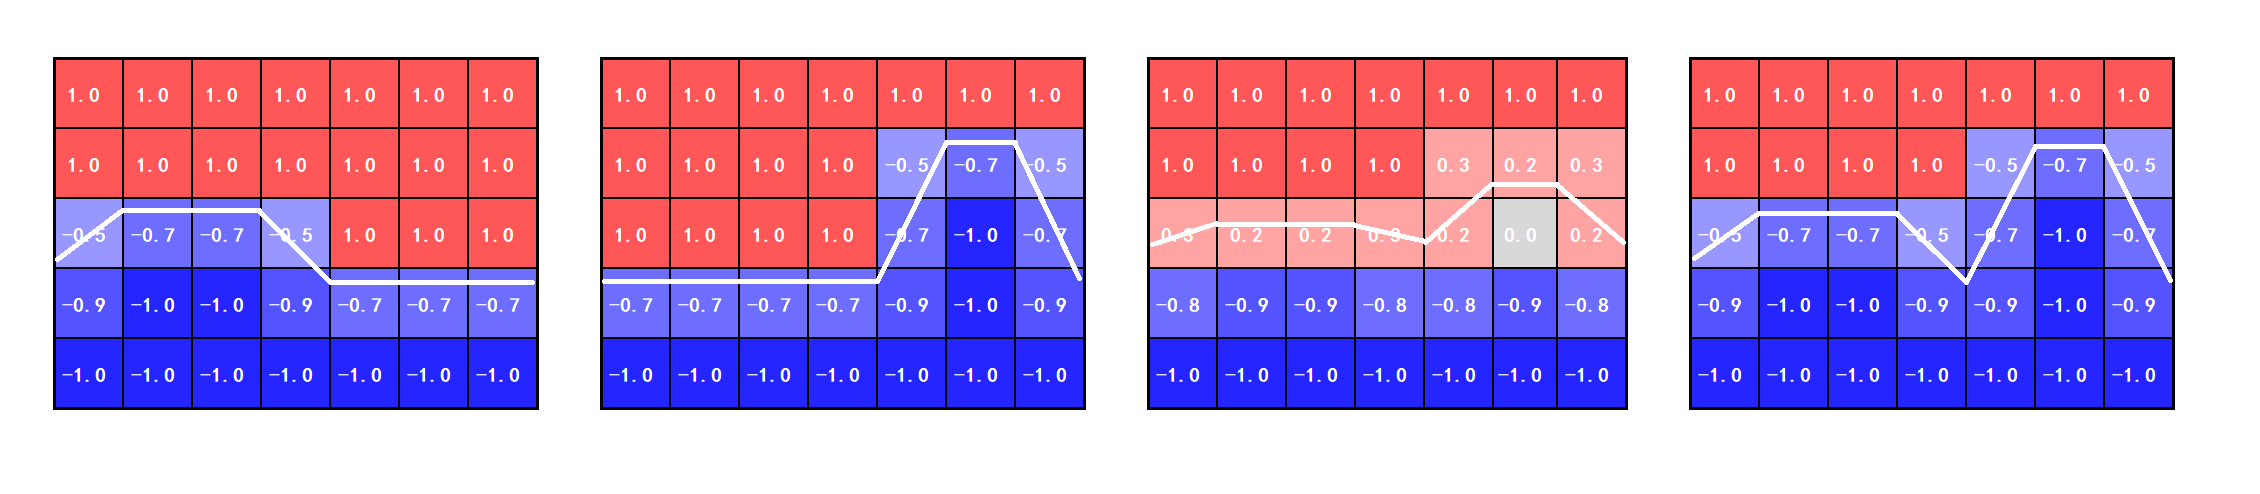
\includegraphics[width=14cm,height=4cm]{figures/figure_tsdf.png}
\setlength{\abovecaptionskip}{-0.5cm}
\caption{Left to right: 1)SDF value from camera 1; 2)Merged SDF value from camera 2; 3)SDF value by simple average; 4)Merged SDF value from our project.}
\label{3}
\end{figure*}
    
Then we use the marching cube to convert the SDF value of each volume to a triangle mesh, which can be done parallelly on GPUs. To fully make use of color images from cameras, we divide one triangle into four triangles by midpoints of each edge. Then we can match color imagine with these triangles for a better texture quality without a large effect on efficiency(Figure YY).

\begin{figure}[H]
\centering
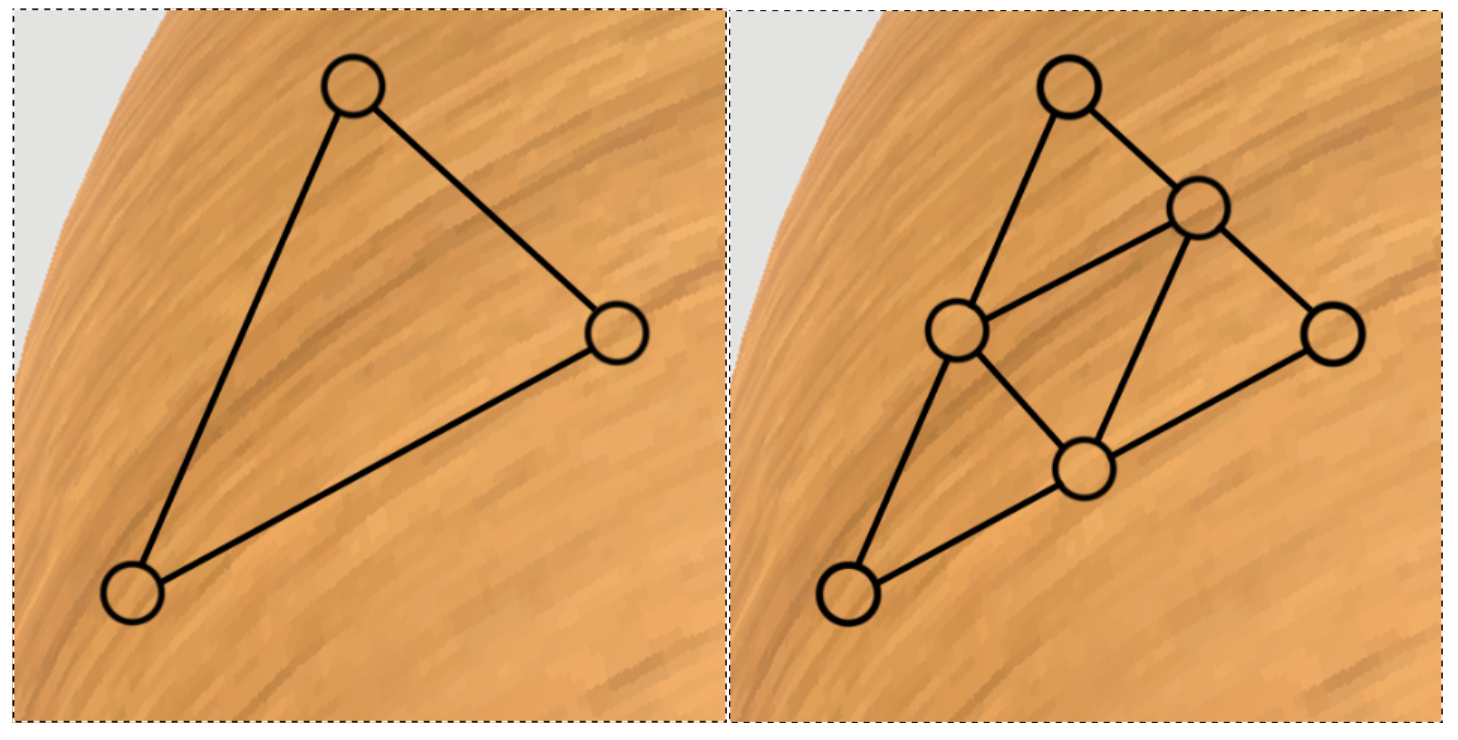
\includegraphics[width=6cm,height=3cm]{figures/figure_mc.png}
\setlength{\abovecaptionskip}{0.5cm}
\caption{Left: Mesh without Supersampling; Right: Mesh witht Supersampling.}
\label{4}
\end{figure}


\subsection{Delay Control}
[from lwq]To gain a more credible result of delay preception in 3DTI, we need have a accurately control over our system. First we synchronize the depth camera array using Realsense SDK. We set the frame rate of cameras at 30FPS and also regard it as the system clock. After that we can start our procession when depth cameras obtain new data. The latency of our system is controllable and it can be minimize to XXXms. Figure XXX shows the pipeline and estimation of latency of our system when using 3 depth cameras each side. To have a better control on the delay, we use a buffer to store the data transmitted from remote client. We can alter the latency by changing the time each set of data remains in the cache.
